\documentclass[12pt, twoside=semi, parskip=half-]{scrartcl}
\usepackage[french]{babel}
\usepackage[T1]{fontenc}
\usepackage[utf8]{inputenc}
\usepackage[sfmath,light, frenchstyle]{kpfonts}
\renewcommand{\familydefault}{\sfdefault}
\usepackage{stmaryrd}
\usepackage{fontawesome5}
\usepackage[margin=1in]{geometry}

\usepackage{mathtools}
\DeclarePairedDelimiter{\abs}{\lvert}{\rvert}
\usepackage{tabularray}
\usepackage{tasks}
\usepackage{graphicx}
\usepackage[export]{adjustbox}
\usepackage{tikzscale}
\usepackage[locale=FR]{siunitx}
\usepackage[use-files]{xsim}
\xsimsetup{
    path=xsim,
    load-style=math-exam,
    solution/print=true
}
\usepackage{tkz-euclide}
\usetikzlibrary{babel}
\begin{document}
\pagestyle{empty}
% PAGE DE GARDE
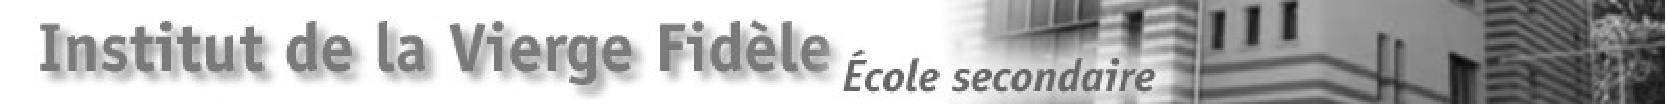
\includegraphics[width=\linewidth]{img/entete.pdf}
    \vspace{\smallskipamount}
    \begin{tblr}{%
            hline{1,3,5,9,10},
            vline{1,4},
            colspec={XXX},%
            cell{1}{1} = {r=1, c=3}{c,font=\bfseries\Huge},%
            cell{2}{1}= {r=1, c=3}{c,font=\bfseries\Large},%
            cell{3}{1}={r=1,c=2}{l},
            cell{4}{1}={r=1,c=2}{l},
            cell{5}{1}={r=1,c=2}{l},
            cell{5}{3}={r=2,c=1}{c},
            cell{6}{1}={r=1,c=2}{l},%
            cell{7}{1}={r=1,c=3}{l},%
            cell{8}{1}={r=1,c=3}{l},%
            row{9}={c},
            rowsep=1ex%
        }%
        % cell1
        UAA5 &&\\
        % cell2
        Similitude et Thalès&&\\
        % cell3
        Nom : && Classe : \\
        % cell4
        Prénom : && Numéro :  \\
        % cell5
        Professeur :  &&\hspace*{1cm}\slash\TotalExerciseGoal{points}{}{}\\
        % cell6
        Date et heure: Vendredi 12 juin 2023 &&\\
        % cell7
        Matériel autorisé : calculatrice &&\\
        % cell8
        Matériel à distribuer : feuille à en-tête, feuille de brouillon&&\\
        % cell9
        C1 : \qquad/\TotalExerciseTypeGoal{connaitre}{points}{}{}
        &
        C2 : \qquad/\TotalExerciseTypeGoal{appliquer}{points}{}{}
        &
        C3 : \qquad/\TotalExerciseTypeGoal{transferer}{points}{}{}\\
    \end{tblr}%
    \vspace{\smallskipamount}
    \begin{scriptsize}%
        Rue de linthout, 30 - 1030 Bruxelles%
    \end{scriptsize}%
    \par%
    \minisec{Quelques consignes}
\begin{itemize}
    \item Rendre une copie soignée et aérée.
    \item Respecter les conventions mathématiques et les notations.
    \item Détailler tous ses raisonnements, la réponse seule ne suffit pas.
    \item Pour les problèmes, n'oubliez pas de formuler la réponse finale  avec une phrase complète.
    \item Arrondir les réponses finales (pas d'arrondis sur les réponses intermédiaires) au centième près.
\end{itemize}
\faIcon{exclamation-triangle} Tout manquement entraînera une perte de points, soyez vigilant lors de la relecture.
\vfill
\begin{flushright}
    Bon travail !
\end{flushright}
\cleardoublepage
\pagestyle{plain}
\setcounter{page}{1}

%%%%%%%%%%%%%%%%%%%%%%%%%%%%%%%%%%%%%%%
% EXERCICE
\begin{connaitre}[points=2]
    Les propositions suivantes sont-elles vraies ou fausses ? Justifie dans les deux cas.
    \begin{tasks}
        \task Deux triangles rectangles isocèles sont semblables.
        \task Si \(ABC \sim DEF\) alors \(\dfrac{\abs{AB}}{\abs{DE}} = \dfrac{\abs{EF}}{\abs{BC}} = \dfrac{\abs{AC}}{\abs{DF}}\).
    \end{tasks}
\end{connaitre}
% SOLUTION
\begin{solconnaitre}
    \begin{tasks}
        % \task Faux, son aire est multipliée par 64.
        \task Vrai, ils auront tous les deux un angle droit et des angles de \ang{45} (cas AA).
        \task Faux, si \(ABC \sim DEF\) alors \(\dfrac{\abs{AB}}{\abs{DE}} = \dfrac{\abs{BC}}{\abs{EF}} = \dfrac{\abs{AC}}{\abs{DF}} = k\).
    \end{tasks}
\end{solconnaitre}
%%%%%%%%%%%%%%%%%%%%%%%%%%%%%%%%%%%%%%%
% EXERCICE
\begin{connaitre}[points=1]
    Les droites \(BE\) et \(CF\) sont-elles parallèles ? Justifie.
    \hfil
  \includegraphics[width=.3\linewidth]{tikz/C1_reciproque_02.tikz}
\end{connaitre}
% SOLUTION
\begin{solution}
    
\end{solution}
%%%%%%%%%%%%%%%%%%%%%%%%%%%%%%%%%%%%%%%
% EXERCICE
\begin{connaitre}[points=1]
    Associe un rapport de similitude à chaque paire de figures semblables.
    \begin{tasks}[label=](4)
        \task \(k_1 = \frac{4}{9}\)
        \task \(k_2 = \frac{3}{2}\)
        \task \(k_3 = \frac{2}{3}\)
        \task \(k_4 = \frac{27}{8}\)
    \end{tasks}
    \begin{tasks}(2)
        \task 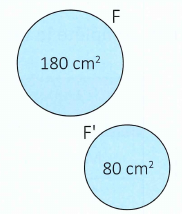
\includegraphics[valign=t,width=.5\linewidth]{img/C1_figures_semblables_02.png}
        \task 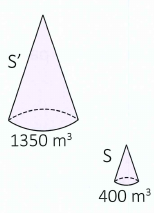
\includegraphics[valign=t,width=.5\linewidth]{img/C1_figures_semblables_03.png}
    \end{tasks}
\end{connaitre}
% SOLUTION
\begin{solconnaitre}
    \begin{tasks}
        \task \(k_4\)
        \task \(k_1\)
    \end{tasks}
\end{solconnaitre}

%%%%%%%%%%%%%%%%%%%%%%%%%%%%%%%%%%%%%%%
% EXERCICE
\begin{appliquer}[points=3]
    Déterminez les longueurs demandées pour chacune des figures ci-dessous. Justifiez rigoureusement (cas de similitude, parallélisme, etc.) et soyez complet.
    \begin{tasks}(2)
        \task \includegraphics[width=\linewidth]{tikz/C2_figures_02_v2.tikz}
        \task \(AB \sslash CD\)\\
        \includegraphics[width=.75\linewidth]{tikz/C2_figures_03.tikz}
    \end{tasks}
\end{appliquer}
% SOLUTION
\begin{solappliquer}
    \begin{tasks}
        \task $ABC \sim DEF$ ?
        $
            \begin{aligned}[t]
                \dfrac{\abs{AC}}{\abs{DF}}
                 & = \dfrac{2}{4,2} \\
                 & = \dfrac{20}{42} \\
                 & = \dfrac{10}{21} \\
            \end{aligned}
            \hfil
            \begin{aligned}[t]
                \dfrac{\abs{AB}}{\abs{DE}}
                 & = \dfrac{3}{6,3} \\
                 & = \dfrac{30}{63} \\
                 & = \dfrac{10}{21} \\
            \end{aligned}
            \hfil
            \begin{aligned}[t]
                \dfrac{\abs{BC}}{\abs{EF}}
                 & = \dfrac{4}{8,4} \\
                 & = \dfrac{40}{84} \\
                 & = \dfrac{10}{21}
            \end{aligned}
        $\bigbreak

        Par le cas CCC, $ABC \sim DEF$. Donc $\abs{\widehat{D}} = \abs{\widehat{A}} = \ang{104}$.
        \task
        $
            \begin{aligned}[t]
                CD \sslash AB \Rightarrow
                \dfrac{\abs{AE}}{\abs{ED}} & = \dfrac{\abs{EB}}{\abs{EC}}
                \qquad\text{Par le théorème de Thalès}                    \\
                \dfrac{x}{9}               & = \dfrac{3}{5}               \\
                x                          & = 9\cdot\dfrac{3}{5}         \\
                x                          & = \dfrac{18}{5}              \\
                x                          & = 3,6
            \end{aligned}
        $
    \end{tasks}
\end{solappliquer}

%%%%%%%%%%%%%%%%%%%%%%%%%%%%%%%%%%%%%%%
% EXERCICE
\begin{transferer}[points=2]
    On veut réduire la taille de la flèche \(RE\).

    Pour cela, on réalise le schéma ci-après dans lequel \(RE \sslash R'E'\).
    \begin{center}
        \includegraphics[width=.5\linewidth]{tikz/C3_fleche_01.tikz}
    \end{center}

    \begin{tasks}
        \task Calculer la longueur de la flèche réduite \(R'E'\).
        \task Quel est le coefficient de réduction ?
        \task En utilisant le même schéma, on veut obtenir une flèche \(R''E''\) dont la longueur est la moitié de la flèche de départ \(RE\). À quelle distance de \(O\) sera placé le nouveau point \(E\) ?
    \end{tasks}

\end{transferer}
% SOLUTION
\begin{soltransferer}
    
\end{soltransferer}
%%%%%%%%%%%%%%%%%%%%%%%%%%%%%%%%%%%%%%%
% EXERCICE
\begin{transferer}[points=1]
    À l'aide des informations sur le dessin ci-dessous. Détermine la profondeur du trou.
    
   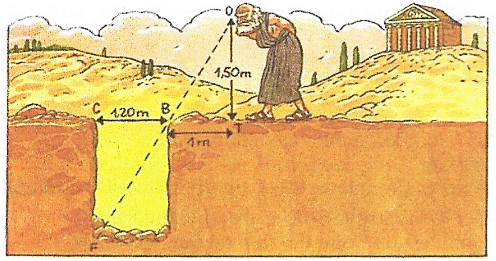
\includegraphics[width=\linewidth]{img/C3_puits.png}
\end{transferer}
% SOLUTION
\begin{soltransferer}
    
\end{soltransferer}
\end{document}